\documentclass{article}
\usepackage[english]{babel}
\usepackage[utf8]{inputenc}
\usepackage[T1]{fontenc}
\usepackage{hyperref}
\usepackage[margin=0.5in]{geometry}
\usepackage{xspace}
\usepackage{xcolor}
\usepackage{amsmath}
\usepackage{graphicx}
\usepackage{palatino}
\usepackage{microtype}

\title{Susceptible-Infected Models for Spatial Vector-Borne Disease}
\author{Drew Dolgert}
\date{\today}


\begin{document}
\maketitle

\section{Introduction}
Approximately seven million people have Chagas disease. It's important.

The causative agent for Chagas disease, T.\ cruzi, is spread by
an insect called Triatoma infestans. The basic model is that 
T.\ infestans spreads Chagas among people and animals in a house.
In order for another household to catch the disease, either people
or the T.\ infestans travel to neighboring houses.
There are three levels, behavior of people, infestation by
T.\ infestans, and spread of T.\ cruzi by T.\ infestans and people.

Mike Levy's group has collected excellent data on the spread of
T.\ infestans in a city. The data are observations of the observed
abundance of insects in households, taken during different sweeps.
All of the work to record abundance amounts to a partially-observed
single trajectory of the system, taken as a whole.

Given that single trajectory of the T.\ infestans through a city,
we would like to ask how behaviors of the insects affect spread
of infestation because this could help intervention against
T.\ infestans. Mike Levy's group previously published a paper
which observed clustering of observations within city blocks,
indicating the insects are less likely to cross roads when
they emigrate a house.

Now we would like to infer from the observed trajectory
to what extent roads affect bug movement. That is a spatial
trajectory defined by bug movement. It is one trajectory
among a combinatorial number of ways T.\ infestans could spread
through the city. We don't have a likelihood for that trajectory,
but we could write a likelihood for an equivalent simplified model.

The simplified model assigns to each house either the state
susceptible or the state infested. Spread from house to house
is assumed to have a uniform hazard within a cutoff distance
and a much smaller hazard at distances greater than the cutoff.
This simplified model, dubbed hop-skip-jump, is a maximum
entropy assumption.

Our concern is that a model which labels the state of the
house will combine several insect behaviors into more
coarse-grained house-infestation behaviors, smearing out
how insect vector movement affects where infestation spreads.
We want to distinguish movement of bugs from stochastic
die-off of populations of T.\ infestans in a house.

This article constructs the simplified \textsc{si} model
rationally from a model of individual T.\ infestans. It uses
a Verhulst model for the insects and establishes a projection
to the more coarse-grained \textsc{si} description.


%%%%%%%%%%%%%%%%%%%%%%%%%%%%%%%%%%%%%%%%%%%%%%%%%%%%%%
\section{Models}
\subsection{Hop-skip-jump Movement Model}
The hop-skip-jump model is a kernel-based movement model
which assigns uniform distributions to the rate for
movement within annuli around the source of infestation.
For this discussion, it's just a hop and a skip, assigning
one rate within a cutoff distance and a much lower rate outside
of it.

All of the models in this article model rates with hazard rates,
the probability of movement given that movement has not yet
happened. Having said rates are constant within a cutoff,
there are two choices for normalization of these rates.
One sets all hazards between houses within the cutoff to the
same value. This feels simple, in line with a notion of
maximum entropy.
The other counts the number of houses within
the cutoff distance and apportions a total hazard evenly
among houses within the cutoff. This would be appropriate
if the movement model expresses a total number of bugs leaving
a single house.

The difference between no normalization and per-house normalization
isn't great if the count of houses within the cutoff doesn't
change greatly. Given the large cutoff distance used in 
previous articles, this is the case for the given dataset.
The constant hazard is also the only version used in previous
literature, so that's what is used below.

Previous work showed streets are important. The tendency
for bugs not to cross streets will be incorporated by counting
the number of street crossings required to walk directly from
one house to another and, for each crossing, multiplying
the hazard for movement by a factor. Using a factor, rather
than a subtraction of a value, follows the literature on
risk modeling.


\begin{figure}
\centerline{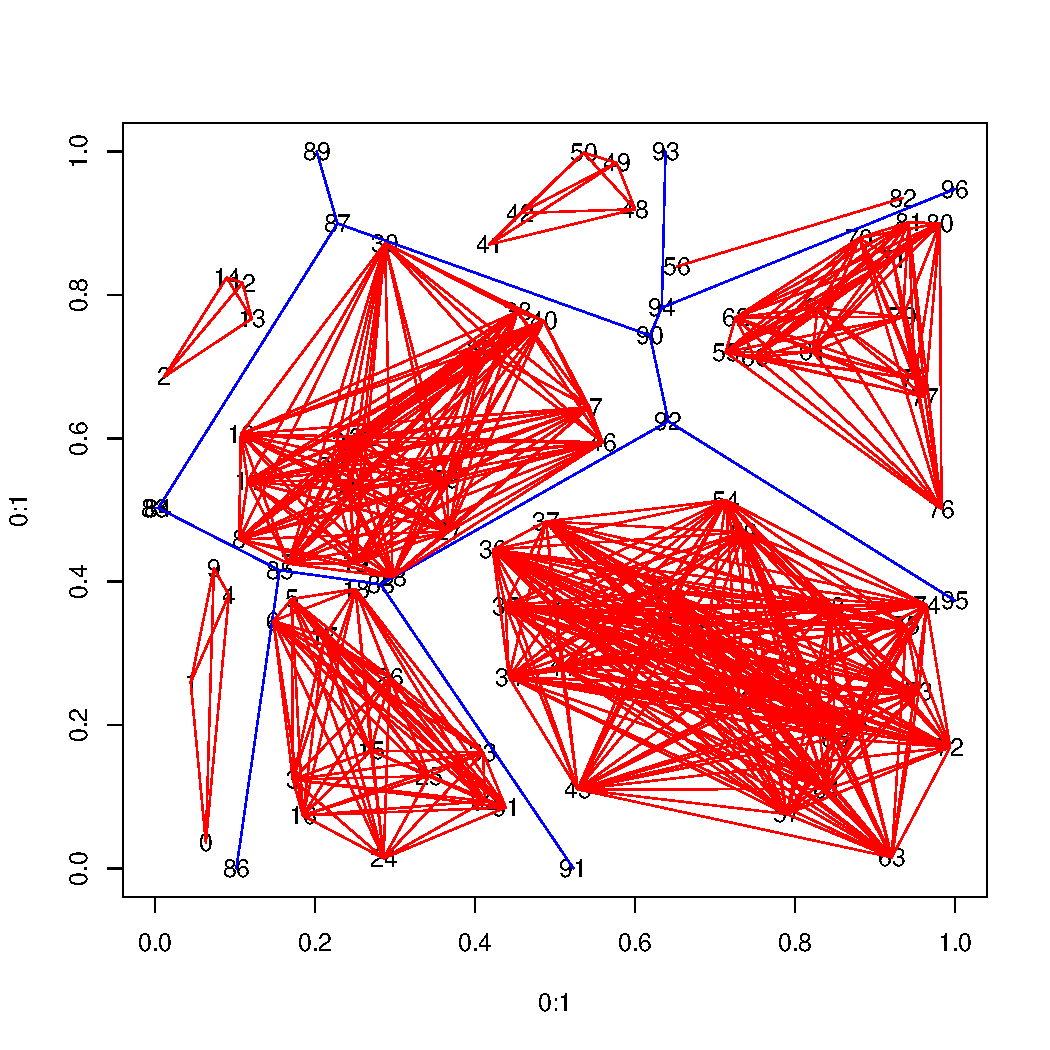
\includegraphics[width=10cm]{blocks.pdf}}
\caption{Houses on different blocks are separated by streets.
Calculate the number of streets crossed by walking house-to-house.
The red lines show paths that do not include streets,
just to prove the street crossing is calculated correctly.\label{fig:blocks}}
\end{figure}

%%%%%%%%%%%%%%%%%%%%%%%%%%%%%%%%%%%%%%%%%%%%%%%%%%%%%%
\subsection{Explicit Spatial Vector Movement Model}
It would be possible to construct a colony growth and
vector movement model for T.\ infestans from expert opinion.
The goal of this article is to ask how to rationally project
any model of individual vectors onto a coarser model.
We choose an underlying vector model which preserves
our preference not to assume what we don't know.
The underlying model for bug birth and death will be
a Verhulst model. As described in N{\aa}sell\cite{Nasell2001},
the Verhulst model predicts logistic growth of bugs within
a house. This model has one more parameter than the
basic \textsc{si} model, effectively controlling variance in
bug growth.

What we gain by introducing a vector-based model with
almost as few parameters as the coarse-grained model is
that the behaviors of the vector provide inherent structure
to the coarse-grained model. Two specific examples
are the time-dependence of emigration and tendency for
stochastic die-off. Modeling birth
and death of insects will generate not only logistic
growth of a population infesting a house, but nearly-logistic
growth of individuals emigrating that house to form new
colonies. This time-dependence is inherent in the insect-based
model and important for early spread of infestation.
Stochastic die-off will decrease the rate of spread
to neighboring houses and may conflate with inference
about mobility of bugs.

\begin{figure}
\centerline{\includegraphics[width=10cm]{bug_trajectory.png}}
\caption{A single house with a birth and death process mirrors
a logistic model. The black line is an average over the
number of individuals at any time, given that the trajectory
doesn't die off. The blue line is an average of trajectories
that die off. Half of the trajectories die off.\label{fig:bug_trajectory}}
\end{figure}

\begin{figure}
\centerline{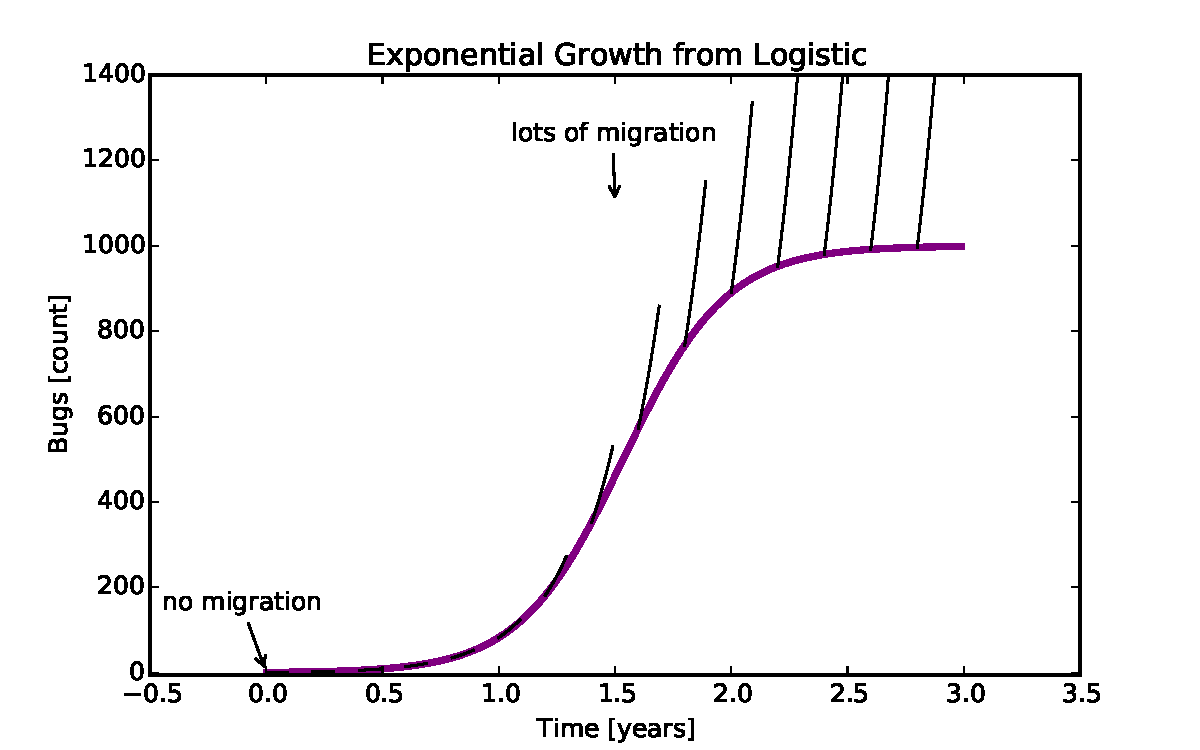
\includegraphics[width=10cm]{excess}}
\caption{Using a portion of excess growth to model
how many bugs move to neighboring houses.\label{fig:excess}}
\end{figure}


\begin{figure}
\centerline{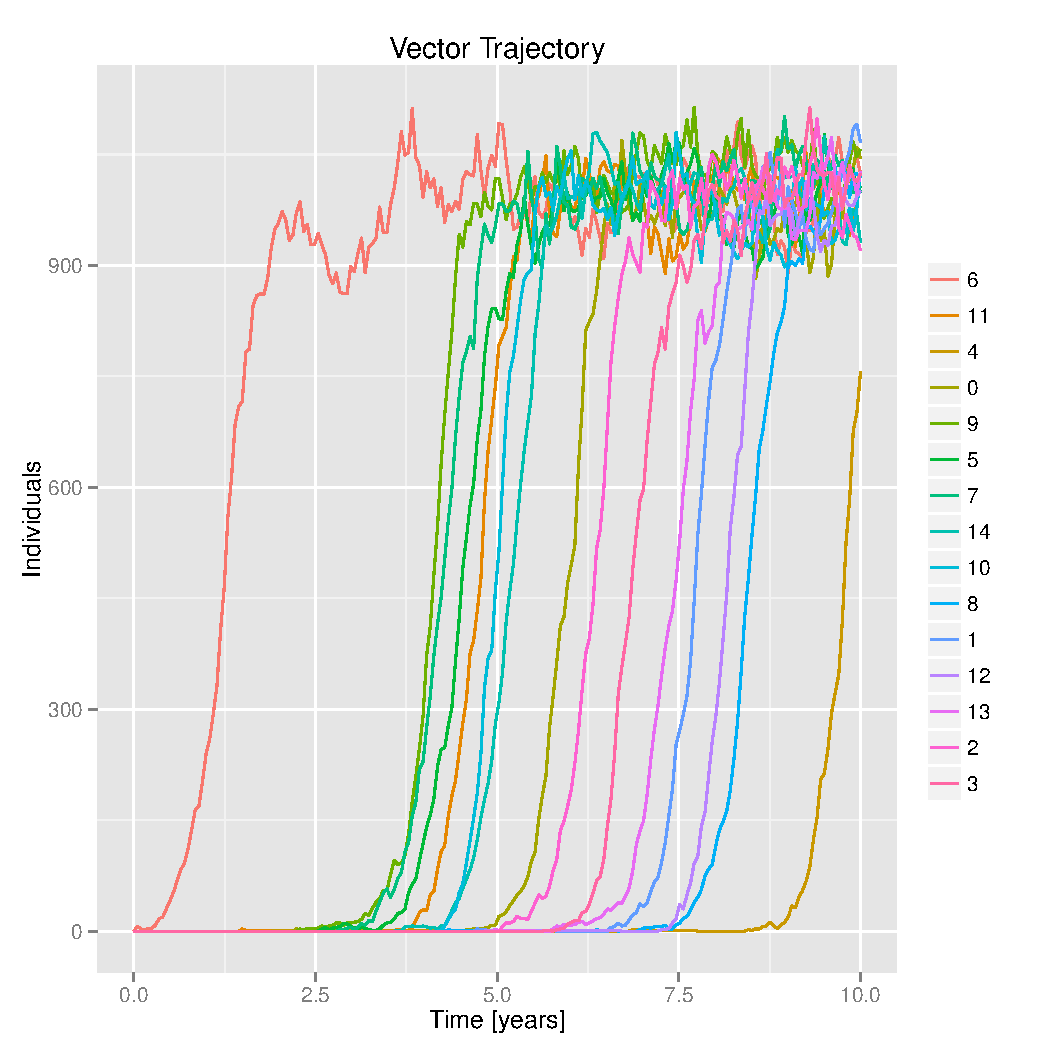
\includegraphics[width=10cm]{housecounts.pdf}}
\caption{For a small simulation of fifteen houses, the vectors increase in number one
individual at a time.\label{fig:housecounts}}
\end{figure}


\begin{figure}
\centerline{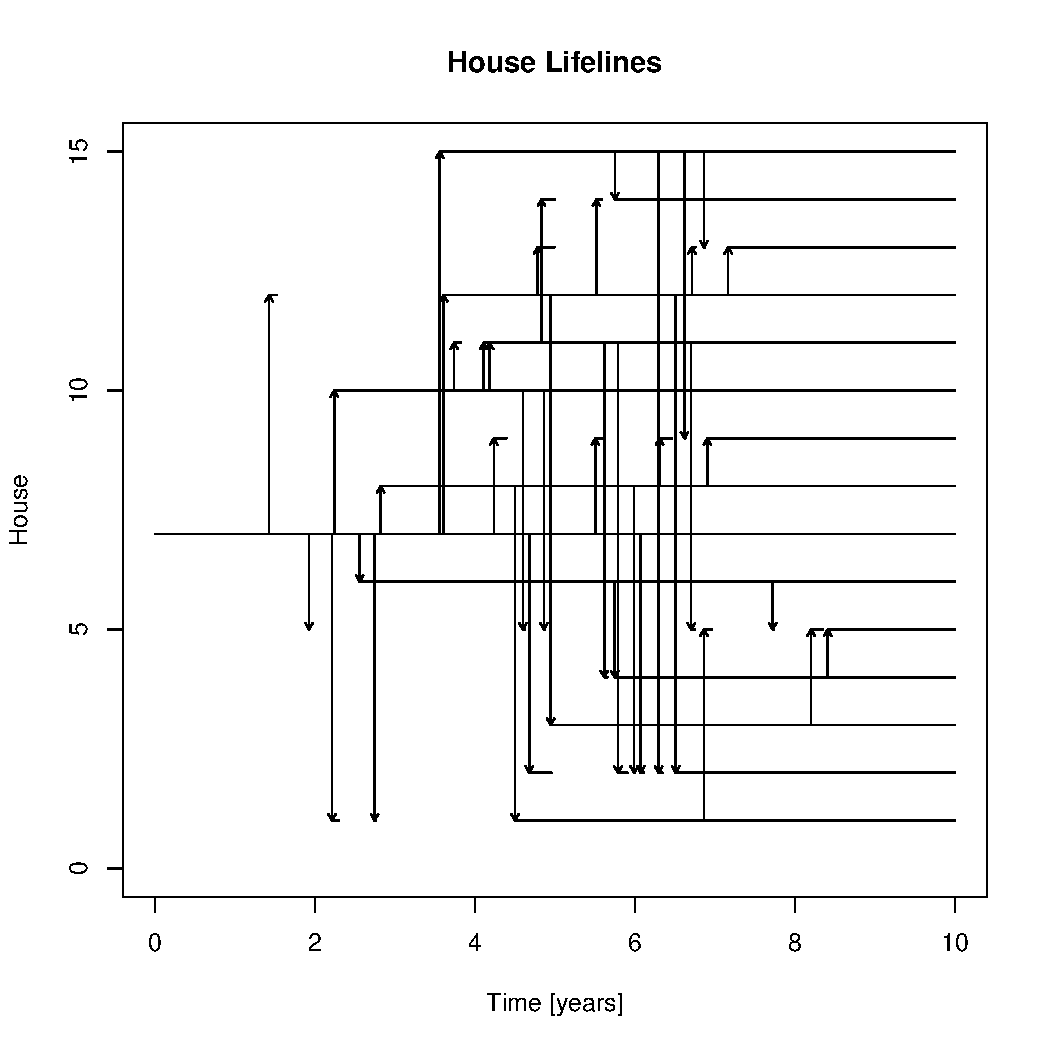
\includegraphics[width=10cm]{houselive.pdf}}
\caption{Stochastic die-off matters a lot for calculation of the
rate of spread. This shows when each house has any bugs in it.
The arrows indicate movement of a bug from one house to another.
Stochastic die-off is shown by lines ending.\label{fig:houselive}}
\end{figure}

Let's first discuss a single household.
The state of the house is $n$, the current number of bugs.
Given $n$, the birth rate and death rate are
\begin{eqnarray}
  \lambda_n & = & \lambda\left(1-\alpha_1\frac{n}{N}\right)n \\
  \mu_n & = & \mu\left(1+\alpha_2\frac{n}{N}\right)n
\end{eqnarray}
with the caveat that, at $n=N$, the birth rate is defined at zero.
This makes the system bounded. $N$ is not the carrying capacity.
The parameters are then $N$, $\lambda$, $\mu$, $\alpha_1$, and $\alpha_2$.

The assumption earlier was that the rate of infestation of
neighbors is proportional to the excess growth rate, which is
$\lambda\alpha_1n^2/N$. Two different ways to understand this
are as a heuristic or as a microscopic model. The heuristic assumes
that excess growth rate results in a higher hazard rate for infestation
of neighbors, meaning the probability of infestation given that the
neighbors aren't yet infested. This excludes re-infestation, or adding
bugs to a house that already has bugs. The microscopic model
sees bugs as leaving one house, dying at a rate, and arriving at neighbors.
In this case, having multiple infested neighbors increases the chance
that early infestation survives stochastic die-off.

This system will have $R_0=\lambda/\mu>1$. In this
case, the carrying capacity is
\begin{equation}
  K_1=\frac{R_0-1}{\alpha_1 R_0+\alpha_2}N.
\end{equation}
The variance on carrying capacity is related to the $\alpha$s,
\begin{equation}
  \sigma_1=\frac{\sqrt{(\alpha_1+\alpha_2)R_0}}{\alpha_1R_0+\alpha_2}\sqrt{N}.
\end{equation}
N{\aa}sell's examples use $\alpha_1=1$ and $\alpha_2=0$. 
Fixing this choice would fix variance in the distribution, given birth
and death rates to determine $R_0$. If there were data on stochastic die-off,
it would inform the choice of these parameters.

Aside from $\alpha_1$ and $\alpha_2$, the rest of the parameters
participate in defining the average logistic curve.
The principle for setting parameters on the Verhulst model
is to assign carrying capacity and time to half maximum infestation,
and then the shape of the curve will come from a reasonable
assumption about the ratio of birth rate to death rate.
Any logistic curve can be written
\begin{equation}
  N(t)=\frac{K_1}{1+\exp\left(-r(t-t_0)\right)}
\end{equation}
where $K_1$ is the carrying capacity, $r$ is a growth rate
which changes the shape of the curve, and $t_0$ is the location
of the midpoint of the curve. The growth rate of a logistic
curve is not the same as the birth rate of a Verhulst model.
Instead, $r=\lambda-\mu$. While $\lambda$ may be understood from lab
experiments, $\mu$ is not. From fieldwork, expert opinion estimates
$t_0$ near a year and the carrying capacity at or above $K_1=1000.$
For a logistic growth model,
the midpoint is $t_0=\ln(K_1/N(0)-1)/r$.Given the Verhulst model
moves single bugs, $N(0)=1$, so $r=\ln(K_1-1)/t_0\approx 7$.
The ration $R_0=\lambda/\mu$ is almost always positive for
ecological models. If we take $R_0=1.5$, then $\mu=2r$ and $\lambda=3r$.
The Verhulst maximum count, $N=K_1R_0/(R_0-1)$. For the given $R_0$,
this is $N=3K_1$.


The desired movement model for a set of houses, each of which
is modeled by a Verhulst model, is to use the excess growth,
proportional to $\lambda \alpha_1 n^2/N$. Instead of picturing
the survival of wandering bugs, remain consistent with the
hop-skip-jump model and assign a maximum hazard rate,
achieved when a house is at carrying capacity, so
$\beta_0=\alpha_3\lambda K_1^2/N$, which leads to
$\alpha_3=3\beta_0/K_1$. The $\beta_0$ parameter says
that a fully infested house is likely to send a bug
to a neighboring house at the given rate per year.
Once every two weeks means $\beta_0=52/2$ if time is measured
in years.

Including movement in a Verhulst model requires forbidding
influx of individuals if the count of individuals is at $N$.
This is sufficiently larger than carrying capacity not to have
an effect.

Stochastic die-off measures the fraction of populations which
start with one individual and then arrive at a state with zero
individuals. For $R_0=1.5$, that fraction is $1/2$.
For a simulation of movement, multiple new arrivals may occur
at nearly the same time, so that the stochastic die-off estimated
from a single arrival is too high. This is especially true
later in a simulation as movement pressure increases.

Plot the stochastic die-off fraction, measured from
a simulation that's a movement model. It will be less because
of multiple importations. Later infestations will have
smaller die-off, too. Use a model of a single colony
with a Poisson-distributed importation rate.

Having an infested neighbor in the same block increases
the likelihood of the first importation. It also increases
the likelihood of survival of the colony because second
importation can happen during early phases.

%%%%%%%%%%%%%%%%%%%%%%%%%%%%%%%%%%%%%%%%%%%%%%%%%%%%%%
\subsection{Susceptible-infested House Model}



%%%%%%%%%%%%%%%%%%%%%%%%%%%%%%%%%%%%%%%%%%%%%%%%%%%%%%
\section{Coarse-Graining by Projection}
Given the model for behavior of individual vectors, construct a 
model for behavior of house infestations.

\begin{tabular}{ll}
Model & Projection \\
SI & A house is infested if vectors would last past stochastic die-off. \\
SIS & A house is infested if there is one bug. \\
SI constant & Constant hazard rate for infectiousness. \\
SNI & Add a stage counting individuals until past stochastic die-off.
\end{tabular}

Fidelity of coarse-grained model over long times.
Fidelity of coarse-grained model for early outbreaks.



\section{Likelihood of Trajectory}
Given a measured trajectory, what is the likelihood using
a coarse-grained model, derived from the vector model?

\begin{itemize}
\item Using MLE on log-likelihood trajectories.
\item Using synthetic likelihood and MCMC.
\item Using ABC?
\end{itemize}


\bibliographystyle{plain}
\bibliography{vectored}
\end{document}
